\chapter{Desenvolvimento do Trabalho} \label{cap:desenvolvimento}
\section{Atividades Previstas}

\subsection{Implementação da infraestrutura}

A infraestrutura foi implementada em três componentes: o firmware do nó sensor, o firmware do \textit{gateway} e o \textit{backend} de persistência, além de ferramentas de análise. Os dois firmwares rodam em placas Heltec WiFi LoRa 32 V3 \cite{heltec_wifi_lora_32_v3}, que integram o microcontrolador ESP32-S3 e o transceptor LoRa SX1262 \cite{semtech_sx1262}. O código está em repositório público, com os registros de decisão que documentam cada escolha e as alternativas descartadas.

Os parâmetros de rádio, o formato do quadro e a chave de rede ficam em um único cabeçalho compartilhado pelos dois firmwares. A escolha é deliberada: uma divergência de frequência, fator de espalhamento ou disposição de bytes entre nó e \textit{gateway} não produz erro de compilação nem mensagem em tempo de execução, apenas um receptor que não recebe nada. Verificações em tempo de compilação garantem que o quadro tem exatamente 26 bytes e não excede o limite de 51 bytes do plano regional.

O nó transmite um quadro a cada cinco segundos, com agendamento em tempo absoluto: o instante da próxima transmissão é calculado a partir do anterior, e não a partir do fim da transmissão corrente, de modo que o tempo de processamento não se acumula como atraso. O contador de quadros é persistido na memória não volátil em blocos de 32: o nó grava o teto do bloco antes de usá-lo e, ao reiniciar, retoma do próximo bloco. Alguns valores são pulados a cada reinício, mas nenhum se repete, o que preserva a unicidade do \textit{nonce} derivado do contador. Os dados de aplicação (temperatura e iluminância) são, nesta etapa, sintéticos: senoides com período conhecido, o que permite verificar a decifragem no receptor por inspeção. Os metadados de recepção, que são as variáveis dos modelos, não dependem deles.

O \textit{gateway} divide o trabalho entre os dois núcleos do processador. No primeiro, uma interrupção do transceptor sinaliza cada quadro recebido; o firmware lê o pacote, registra RSSI e SNR, recoloca o rádio em escuta e só então valida o quadro, na ordem do LoRaWAN: verifica a janela anti-replay pelo contador em claro, autentica e decifra, e apenas depois de a autenticação conferir avança a janela. O registro JSON com os doze campos sai pela interface serial antes de qualquer envio pela rede, sob exclusão mútua para que nenhum diagnóstico o corte ao meio. O quadro é então depositado, sem espera, em uma fila para o segundo núcleo. Nesse núcleo, uma tarefa mantém a conexão Wi-Fi e a sincronização de relógio por NTP, agrupa os quadros em lotes de até vinte, envia ao \textit{backend} e, em caso de falha, guarda até 512 registros e tenta novamente com espera crescente de 1 a 30 segundos. Cada quadro entregue mais de quinze segundos após a recepção é marcado como reenviado, e o instante UTC de recepção é reconstruído a partir do relógio monotônico do dispositivo, de modo que quadros recebidos antes da sincronização de relógio saem com hora correta. A cada trinta segundos o \textit{gateway} emite um sinal de vida com os contadores de quadros recebidos, rejeitados por replay, por autenticação e por CRC, e com o estado da fila e da conexão.

O \textit{backend} é uma API em FastAPI com banco SQLite. A rota de ingestão valida cada quadro contra um esquema que rejeita campos desconhecidos, para que um nome de campo errado produza um erro imediato em vez de uma coluna perdida, e insere com um índice único sobre \textit{gateway}, sessão, dispositivo e contador, o que torna o reenvio idempotente. Rotas de consulta devolvem quadros, resumo por sessão e agregados de uma sessão, e uma página de monitoramento servida pela própria API exibe, em tempo quase real, as séries de RSSI, SNR e intervalo, com marcas nos reinícios do nó. A separação entre salto por reinício e perda de rádio, descrita na Seção~\ref{sec:resultados_infra}, é feita por um módulo único, usado tanto pela API quanto pela ferramenta de análise do registro serial, para que as duas fontes nunca discordem. O \textit{backend} tem dezoito testes automatizados.

Quatro suítes de teste acompanham o firmware, executadas na própria placa: verificação de inicialização (pinos, transceptor, potência de bancada), codificação e decodificação do quadro com rejeição de quadros forjados, formatação byte a byte do registro JSON e persistência do contador. A primeira foi executada nas duas placas; as outras três compilam e sua execução no hardware está pendente.



%%%%%%%%%%%%%%%%%%%%%%%%%%%%%%%%%%%%%%%%%%%%%%%%%%%%


\subsection{Segurança com Ascon}
A camada de segurança foi desenvolvida em cinco atividades, cujos resultados estão na Seção~\ref{sec:resultados_ascon}. A biblioteca \textit{ascon-suite} foi integrada ao ambiente do ESP32 e, sobre ela, foi escrita a biblioteca \textit{AsconSecure}, que cifra e autentica o \textit{payload} de cada mensagem antes de entregá-lo ao rádio. A implementação foi validada pelos \textit{Known Answer Tests} oficiais, de forma exaustiva no computador e com um subconjunto na própria placa. A chave de cada nó passou a ser gerada no próprio dispositivo durante o provisionamento, pelo gerador de hardware do ESP32 com o CTR\_DRBG da \textit{mbedTLS}, seguindo as recomendações do NIST. Uma bateria de adulteração com 4.907 casos, sobre o texto cifrado, os dados associados, a \textit{tag} e o \textit{nonce}, confirmou que toda mensagem alterada é rejeitada. Por fim, mediram-se o tempo de execução em ciclos de \textit{clock}, a memória de \textit{heap}, pilha e \textit{Flash}, o tempo constante e o comparativo com o AES-128-GCM nas duas placas, e o consumo de energia com resistor \textit{shunt} e osciloscópio no ESP32 clássico.

%%%%%%%%%%%%%%%%%%%%%%%%%%%%%%%%%%%%%%%%%%%%%%%%%%%%

\subsection{Modelo de Machine Learning}

O desenvolvimento da frente de aprendizado de máquina seguirá um conjunto de
atividades voltadas à preparação dos dados, treinamento dos modelos e avaliação
da capacidade de detecção de anomalias. O objetivo dessa etapa é construir uma
base experimental consistente para comparar diferentes abordagens de regressão
temporal aplicadas ao comportamento da rede LoRaWAN.

As atividades previstas para essa frente de trabalho são:
\begin{itemize}
    \item \textbf{Preparação dos datasets:} Organizar os dados selecionados para a etapa de modelagem, com foco principal no dataset Tour Perret e uso complementar do dataset GUARD. Essa preparação incluirá harmonização de timestamps, tratamento de valores ausentes, extração dos atributos relevantes e organização das observações por dispositivo.

    \item \textbf{Definição e seleção de variáveis:} Avaliar os atributos disponíveis nos datasets e selecionar o subconjunto de variáveis mais adequado para a modelagem temporal do comportamento normal da rede. Entre os candidatos principais estão RSSI, SNR, FCnt, \textit{inter-arrival time} e \textit{data rate}, considerando sua estabilidade temporal, disponibilidade e relevância para a identificação de desvios.

    \item \textbf{Divisão temporal dos dados:} Separar os dados em conjuntos de treinamento (60\%), validação (20\%) e teste (20\%) por meio de uma divisão cronológica, preservando a ordem temporal das observações e evitando vazamento de informação futura para o treinamento dos modelos.

    \item \textbf{Exploração e seleção de arquiteturas:} Implementar os modelos ARIMA, RNN e LSTM definidos na etapa metodológica do trabalho. Para cada modelo, será realizada uma exploração de hiperparâmetros e configurações arquiteturais com o objetivo de identificar combinações adequadas ao problema. A seleção de configurações será orientada por critérios de desempenho preditivo e simplicidade estrutural, priorizando modelos com menor complexidade quando o ganho de performance for marginal.

    \item \textbf{Treinamento exclusivo em dados normais:} Todos os modelos serão treinados e validados exclusivamente com dados representativos da operação normal da rede (dataset Tour Perret), garantindo que o comportamento esperado seja aprendido sem contaminação por anomalias ou ataques.

    \item \textbf{Avaliação da qualidade preditiva:} Comparar os modelos com base em métricas de erro de regressão (MAE e RMSE) no conjunto de teste, com o objetivo de verificar qual abordagem representa com maior fidelidade o comportamento esperado das variáveis monitoradas.

    \item \textbf{Calibração de limiar de detecção:} Com base nos resíduos do conjunto de validação, será definido um critério de limiarização (baseado em desvio padrão ou percentis) para classificar observações como normais ou potencialmente anômalas.

    \item \textbf{Avaliação da capacidade de detecção:} Analisar a performance de detecção dos modelos no conjunto de teste e também na aplicação aos dados do dataset GUARD, com o objetivo de verificar se os modelos conseguem identificar anomalias quando confrontados com padrões diferentes ou com ataques conhecidos. Será utilizada a métrica de teste de generalização para avaliar robustez.

    \item \textbf{Análise de viabilidade para execução em borda:} Após a comparação entre os modelos, será realizada uma análise complementar da complexidade das soluções obtidas, considerando número de parâmetros, custo computacional e compatibilidade com uma eventual etapa futura de adaptação para TinyML.
\end{itemize}

%%%%%%%%%%%%%%%%%%%%%%%%%%%%%%%%%%%%%%%%%%%%%%%%%%%%

\subsection{Integração progressiva da solução}

A integração seguiu os marcos definidos no Capítulo~\ref{cap:metodo}, e a Tabela~\ref{tab:marcos_cronologia} registra quando cada um foi atingido. Os três primeiros marcos, que estabelecem a cadeia de ferramentas, a inicialização do transceptor e o enlace ponta a ponta, foram concluídos com a coleta de referência de 23 de agosto de 2026, com o quadro ainda em claro. O quinto e o sétimo, que acrescentam o envio ao \textit{backend} e o quadro autenticado, foram desenvolvidos em paralelo e validados juntos na coleta de 24 de setembro de 2026, descrita na Seção~\ref{sec:resultados_infra}. Sobre essa base, a frente de criptografia substitui o algoritmo da camada de cifra por uma opção de compilação, sem alterar o restante do firmware, e a frente de aprendizado de máquina consome a base persistida.

\begin{table}[htb]
\centering
\caption{Cronologia dos marcos da infraestrutura}
\label{tab:marcos_cronologia}
\begin{tabular}{clll}
\hline
\textbf{Marco} & \textbf{Objetivo} & \textbf{Data} & \textbf{Estado} \\
\hline
1 & Cadeia de ferramentas & jul. 2026 & concluído \\
2 & Rádio & jul. 2026 & concluído \\
3 & Enlace ponta a ponta & 23 ago. 2026 & concluído \\
4 & Sensores reais & & pendente \\
5 & Wi-Fi, HTTP e API & 24 set. 2026 & concluído \\
6 & Energia & & firmware pronto \\
7 & Segurança do enlace & 24 set. 2026 & Ascon pendente \\
\hline
\end{tabular}
\legend{Fonte: elaborado pelos autores (2026).}
\end{table}

Três dificuldades de integração merecem registro, porque afetam a coleta de dados. A primeira: abrir a porta serial do nó reinicia a placa, pois o conversor USB-serial pulsa as linhas de controle ao abrir a conexão; um reinício no meio da coleta zera a sessão. Desde então o nó opera em bateria e sem monitoramento durante as coletas, e o \textit{gateway} é o único ponto de observação. A segunda: o hotspot de celular usado como rede no laboratório é classificado pelo sistema operacional do servidor como rede pública, o que exige uma regra de firewall explícita para a porta da API. A terceira: o relógio do servidor estava cerca de meio segundo atrás do relógio do \textit{gateway}, sincronizado por NTP, o que impede usar a diferença entre o instante de recepção e o de ingestão como medida de latência sem sincronizar o servidor.


%%%%%%%%%%%%%%%%%%%%%%%%%%%%%%%%%%%%%%%%%%%%%%%%%%%%%%
%%%%%%%%%%%%%%%%%%%%%%%%%%%%%%%%%%%%%%%%%%%%%%%%%%%%%%

\section{Resultados da infraestrutura de comunicação}
\label{sec:resultados_infra}

\subsection{Configuração da bancada e métricas}

As duas placas permaneceram estáticas, a poucos metros uma da outra, em ambiente interno. A Tabela~\ref{tab:parametros_enlace} apresenta os parâmetros do enlace e a razão de cada escolha. O nó foi alimentado por bateria portátil e não foi conectado a computador durante as coletas; o \textit{gateway} registrou cada quadro na serial e, na segunda coleta, também no \textit{backend}. Ao fim de cada coleta, o registro serial e o banco de dados foram conferidos quadro a quadro.

\begin{table}[htb]
\centering
\caption{Parâmetros do enlace e justificativas}
\label{tab:parametros_enlace}
\small
\begin{tabular}{p{3cm}p{2cm}p{9,4cm}}
\hline
\textbf{Parâmetro} & \textbf{Valor} & \textbf{Justificativa} \\
\hline
Frequência & 916,8 MHz & Canal 8 do plano AU915 \cite{lorawan_rp002}, na faixa de 915 a 928 MHz autorizada para radiação restrita \cite{anatel_radiacao_restrita}. \\
SF, BW, CR & 7, 125 kHz, 4/5 & Menor tempo no ar (61,7 ms para 26 bytes). Corresponde ao DR5 do plano AU915. \\
Palavra de sincronismo & 0x12 & Rede privada; o LoRaWAN usa 0x34. Evita recepção cruzada com redes LoRaWAN próximas. \\
Potência & 5 dBm & A poucos metros, potências maiores saturam o receptor e o RSSI deixa de refletir o enlace. Como o RSSI é variável dos modelos, medi-lo saturado contaminaria os dados. A placa admite 22 dBm, reservados ao teste de alcance. \\
Período & 5 s & Agendamento em tempo absoluto, sem acúmulo de atraso. \\
\hline
\end{tabular}
\legend{Fonte: elaborado pelos autores (2026).}
\end{table}

A qualidade do enlace é descrita por quatro métricas, todas derivadas do registro do \textit{gateway}. A \textbf{perda de rádio} é o número de contadores ausentes na faixa observada em uma sessão, excluídos os saltos por reinício do nó: como o contador é persistido em blocos de 32, um reinício o faz avançar para o próximo múltiplo, e os valores pulados nunca foram transmitidos. Um buraco é classificado como reinício quando o novo contador é múltiplo de 32 e o intervalo entre os dois quadros recebidos é menor do que 75\% do intervalo que a perda dos quadros ausentes teria produzido. A \textbf{cadência} é a média e o desvio padrão do intervalo entre quadros de contadores consecutivos; intervalos que atravessam um buraco não entram, e o primeiro quadro de cada sessão tem intervalo nulo, não zero. \textbf{RSSI} e \textbf{SNR} são descritos por média e faixa.

\subsection{Coletas realizadas}

Foram realizadas duas coletas de pelo menos uma hora, resumidas na Tabela~\ref{tab:coletas}. A primeira, em 23 de agosto, validou o enlace com o quadro em claro de 10 bytes e sem \textit{backend}. A segunda, em 24 de setembro, usou o quadro autenticado de 26 bytes, com AES-128-GCM como algoritmo de linha de base, e o \textit{backend} no ar.

\begin{table}[htb]
\centering
\caption{Resultados das coletas em bancada}
\label{tab:coletas}
\begin{tabular}{lrr}
\hline
 & \textbf{Referência, 23/08} & \textbf{Integração, 24/09} \\
\hline
Quadro & 10 bytes, em claro & 26 bytes, autenticado \\
Duração & 82,3 min & 71,5 min \\
Quadros recebidos & 989 & 857 \\
Contadores esperados na faixa & 989 & 890 \\
Pulados por reinício do nó & 0 & 33 \\
Perdidos no ar & 0 & 0 \\
Cadência: média & 5000,00 ms & 4999,98 ms \\
Cadência: desvio padrão & 1,00 ms & 1,56 ms \\
Cadência: faixa & 4999 a 5001 ms & 4996 a 5004 ms \\
RSSI: média & $-24{,}7$ dBm & $-33{,}4$ dBm \\
RSSI: mínimo & $-39$ dBm & $-47$ dBm \\
SNR: faixa & 2,25 dB & 2,50 dB \\
Entregues ao \textit{backend} & não se aplica & 857 de 857, em tempo real \\
\hline
\end{tabular}
\legend{Fonte: elaborado pelos autores (2026).}
\end{table}

\begin{figure}[htb]
  \caption{\label{fig:cadencia_coletas}Intervalo entre quadros consecutivos nas duas coletas}
  \begin{center}
      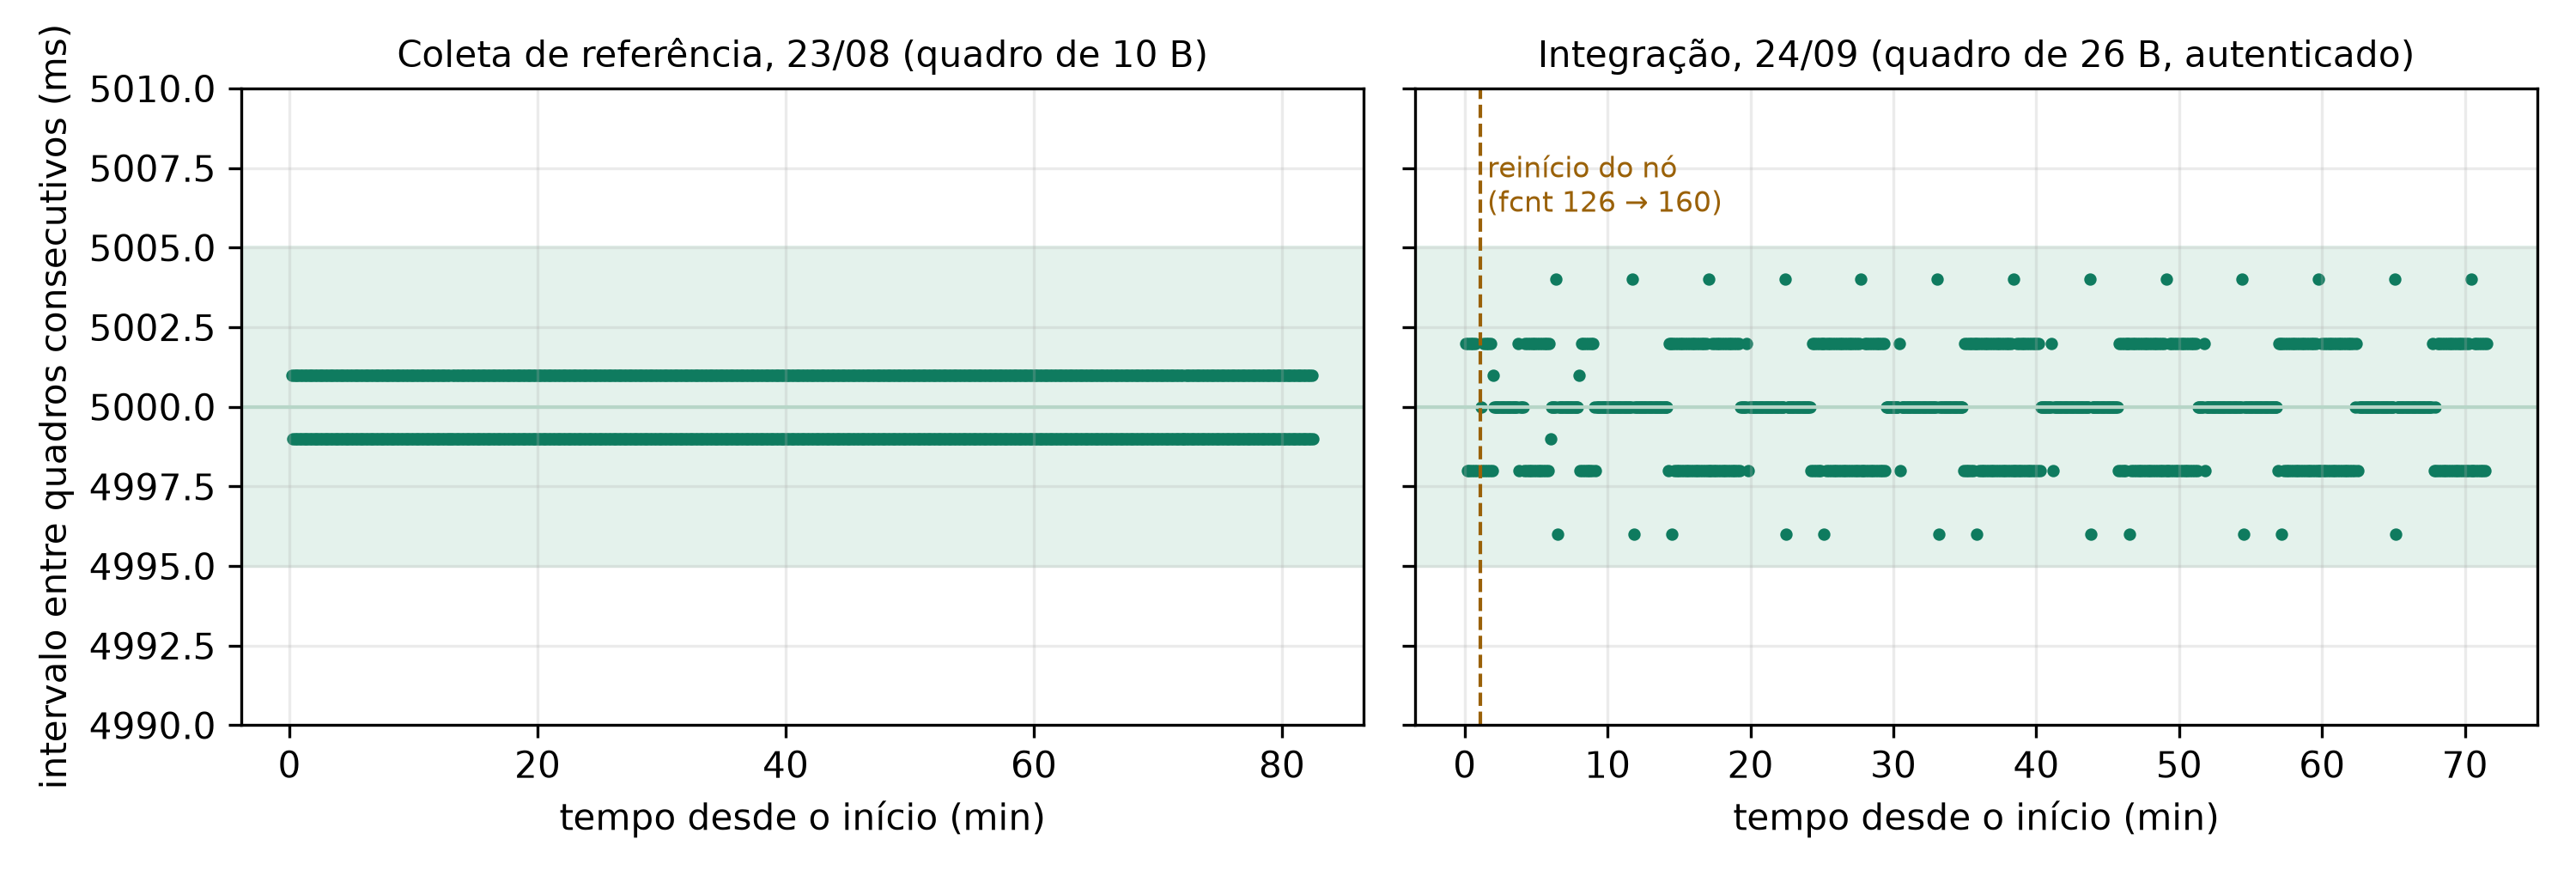
\includegraphics[width=\textwidth]{figuras/cadencia_coletas.png}
  \end{center}
  \legend{Fonte: elaborado pelos autores (2026). A faixa sombreada indica $\pm 5$ ms em torno do período. A linha tracejada marca o reinício do nó.}
\end{figure}

A Figura~\ref{fig:cadencia_coletas} mostra o intervalo entre quadros consecutivos ao longo das duas coletas. Em nenhuma delas houve perda de rádio, e a cadência ficou dentro de $\pm 5$~ms do período em todos os quadros. O desvio padrão maior na segunda coleta (1,56 contra 1,00 ms) é compatível com o processamento adicional nas duas pontas, a cifragem no nó e a atividade de Wi-Fi no 	extit{gateway}, mas atribuí-lo a uma delas exigiria medição dedicada, com carimbo de tempo de microssegundo.

\begin{figure}[htb]
  \caption{\label{fig:rssi_integracao}RSSI por quadro na coleta de 24 de setembro}
  \begin{center}
      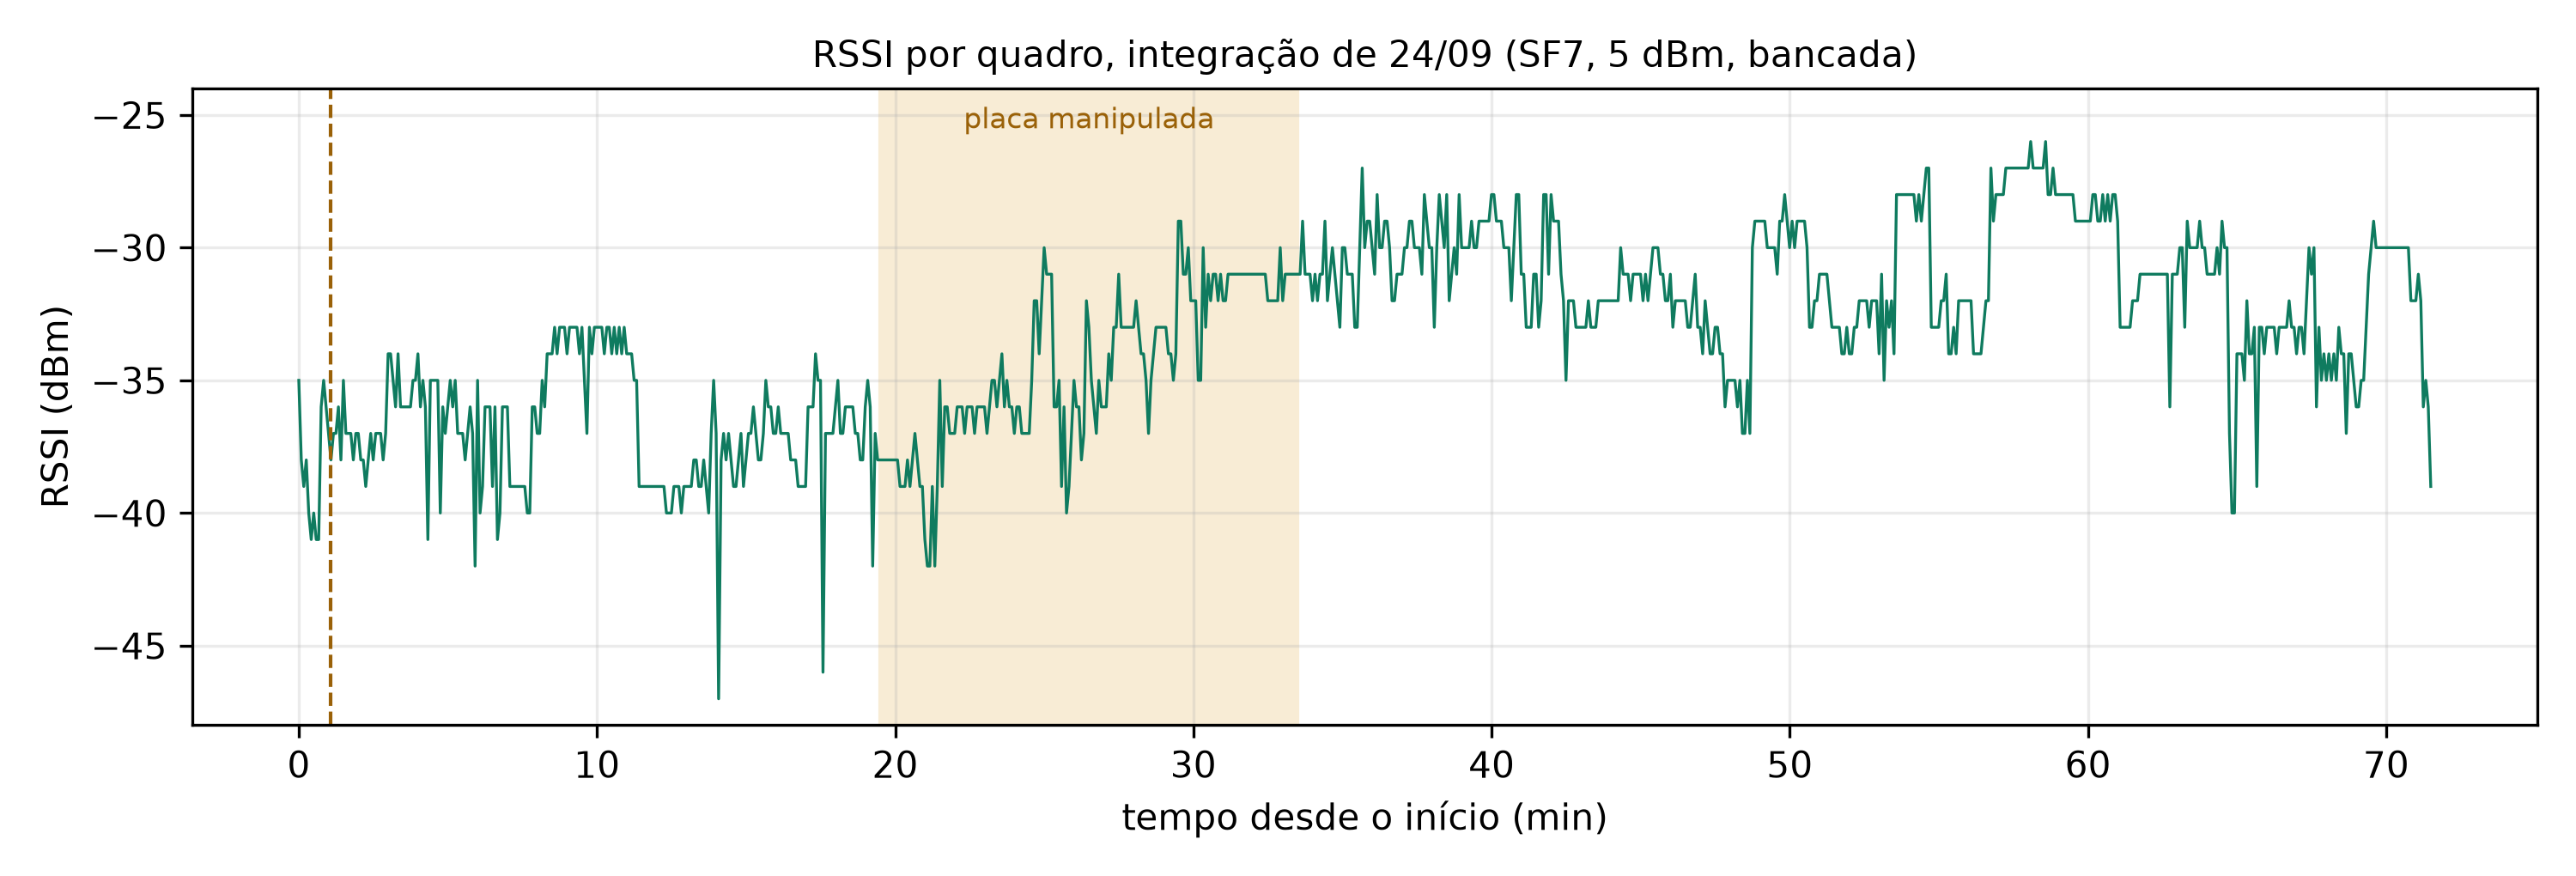
\includegraphics[width=\textwidth]{figuras/rssi_integracao.png}
  \end{center}
  \legend{Fonte: elaborado pelos autores (2026). A área sombreada indica o período em que a placa do nó foi manipulada.}
\end{figure}

\subsection{Discussão}

\textbf{Reinício do nó e perda de rádio.} Na coleta de 24 de setembro, o contador saltou de 126 para 160 com intervalo de 14,7~s entre os dois quadros. Uma contagem simples registraria 33 quadros perdidos, ou 3,7\% de perda. A perda real de 33 quadros teria produzido um intervalo de cerca de 170~s; o intervalo observado e o fato de 160 ser múltiplo de 32 identificam um reinício do nó. A regra que separa os dois casos foi incorporada à API e à ferramenta de análise depois desse achado, e é o motivo de a Tabela~\ref{tab:coletas} distinguir "pulados" de "perdidos". Para a frente de aprendizado de máquina, a distinção importa: um reinício é um evento do dispositivo, uma perda é um evento do enlace, e um detector treinado sem essa separação aprenderia a confundir os dois.

\textbf{Mudança de regime no RSSI.} A Figura~\ref{fig:rssi_integracao} mostra o RSSI em torno de $-37$~dBm nos primeiros vinte minutos e entre $-30$ e $-33$~dBm a partir do trigésimo quarto, com uma transição no intervalo em que a placa do nó foi manipulada. Não é um fenômeno de rede: é a posição da antena. O episódio ilustra o que os modelos precisam distinguir: uma mudança de regime causada por intervenção física produz uma série que um detector de anomalias marcaria, e só o contexto operacional permite rotulá-la corretamente.

\textbf{SNR saturado.} Nas duas coletas o SNR variou menos de 3~dB enquanto o RSSI variou mais de 15~dB, sem correlação entre os dois. Com as placas a poucos metros, o estimador de SNR do transceptor opera saturado, como discutido na Subseção~\ref{subsec:camada_fisica_lora}. Em bancada, o SNR é uma coluna quase constante e não tem valor como variável de entrada; ele só passa a variar de forma útil em testes de alcance.

\textbf{Tempo no ar.} O tempo no ar calculado pela fórmula do fabricante para o quadro de 26 bytes em SF7 é de 61,7~ms, e para o quadro de 10 bytes, 41,2~ms. O tempo medido da função de transmissão, do início da chamada ao fim da transmissão, foi de 69 e 48~ms, respectivamente. A diferença de cerca de 7~ms é constante e corresponde ao processamento fora do rádio: montagem do quadro, cifragem e carga do transceptor. A camada de segurança acrescentou 50\% ao tempo no ar (de 41,2 para 61,7~ms), quase todo devido à tag de autenticação de 16 bytes; derivar o \textit{nonce} em vez de transmiti-lo evitou outros 16 bytes, que elevariam o tempo no ar a 87,3~ms.

\textbf{Limitações.} Uma coleta com perda zero valida a infraestrutura, mas é o caso em que nada está errado: quase toda a variabilidade que um detector precisa aprender está ausente, e as coletas apresentadas servem como referência de comportamento normal, não como conjunto de treinamento. Os dados de aplicação são sintéticos. A janela anti-replay do \textit{gateway} vive em memória volátil: um reinício do \textit{gateway} a zera, e há uma janela de repetição possível até a chegada do primeiro quadro válido, limitação que o LoRaWAN resolve persistindo o contador no \textit{network server}. Todos os nós compartilhariam uma mesma chave, ao contrário do LoRaWAN, em que cada dispositivo tem a sua. A medição de energia do nó e o teste de alcance com fatores de espalhamento maiores não foram executados.


%%%%%%%%%%%%%%%%%%%%%%%%%%%%%%%%%%%%%%%%%%%%%%%%%%%%%%
%%%%%%%%%%%%%%%%%%%%%%%%%%%%%%%%%%%%%%%%%%%%%%%%%%%%%%

\section{Resultados dos Testes da Camada de Segurança (Ascon)}
\label{sec:resultados_ascon}

Esta seção reúne os resultados dos testes de validação e avaliação da camada de segurança baseada no Ascon, seguindo a metodologia definida na Seção \ref{subsec:validacao-ascon}. Os resultados são incorporados de forma progressiva, à medida que cada etapa de teste é concluída.

%%%%%%%%%%%%%%%%%%%%%%%%%%%%%%%%%%%%%%%%%%%%%%%%%%%%%%

\subsection{Validação por \textit{Known Answer Tests} (KAT)}
\label{subsec:kat_resultados}

A validação funcional foi conduzida com os vetores oficiais do Ascon-128a (versão 1.2) distribuídos com a \textit{ascon-suite}. Inicialmente, a biblioteca foi compilada em um computador \textit{desktop} e submetida à execução exaustiva dos 1089 vetores de teste, nos quais cada combinação de chave, \textit{nonce}, dados associados e texto em claro deve produzir um texto cifrado e uma \textit{tag} de autenticação exatos.

Todos os 1089 vetores foram processados com correspondência integral em relação às saídas esperadas, sem nenhuma falha. Como verificação adicional, os vetores foram regenerados a partir da própria implementação e comparados byte a byte com o arquivo de referência, resultando em arquivos idênticos. Por fim, a suíte de testes automatizados (\textit{CTest}) foi executada sobre as variantes em C, C++, \textit{SIV} e mascarada do algoritmo, com aprovação nos 14 casos avaliados. A Tabela~\ref{tab:kat_ascon128a} sintetiza esses resultados.

\begin{table}[htb]
\centering
\caption{Resultado da validação por \textit{Known Answer Tests} do Ascon-128a}
\label{tab:kat_ascon128a}
\begin{tabular}{lrr}
\hline
\textbf{Verificação} & \textbf{Casos} & \textbf{Falhas} \\
\hline
Execução exaustiva (\textit{desktop})                  & 1089 vetores & 0 \\
Regeneração \textit{vs.} referência                    & 1089 vetores & 0 \\
Suíte \textit{CTest} (C, C++, \textit{SIV}, mascarada) & 14 testes    & 0 \\
Execução na placa (ESP32, subconjunto)                 & 6 vetores    & 0 \\
\hline
\end{tabular}
\legend{Fonte: elaborado pelos autores.}
\end{table}

Esses resultados comprovam que a implementação do Ascon-128a opera corretamente no ambiente de desenvolvimento, reproduzindo de forma exata os valores de referência do algoritmo.

Confirmada a correção em \textit{desktop}, um subconjunto representativo dos vetores foi executado diretamente na placa ESP32, cobrindo os limites de processamento por blocos: entrada vazia, bloco parcial, bloco completo e múltiplos blocos, com e sem dados associados. Para cada vetor, verificaram-se tanto a cifração, comparando o resultado com o valor de referência, quanto a decifração, confirmando a recuperação do texto claro com a \textit{tag} validada. Os seis vetores foram reproduzidos com correspondência integral na placa, descartando divergências introduzidas pela compilação ou pela arquitetura do \textit{hardware} (Xtensa LX, \textit{little-endian}). Nessa execução, o estado interno do algoritmo (\texttt{ascon128a\_state\_t}) ocupou 80 bytes, valor retomado posteriormente na análise de memória.

Os vetores utilizados e o registro completo das execuções, em \textit{desktop} e na placa, estão disponíveis no repositório do projeto, na pasta \texttt{kat-validation}.

%%%%%%%%%%%%%%%%%%%%%%%%%%%%%%%%%%%%%%%%%%%%%%%%%%%%%%

\subsection{Validação dos Dados Associados (AEAD)}
\label{subsec:aead_resultados}

A propriedade de autenticação do modo AEAD foi avaliada por injeção intencional de falhas, simulando um atacante que intercepta e altera a mensagem em trânsito. A partir de um pacote válido, cada adulteração foi aplicada isoladamente e a mensagem resultante submetida à decifragem, que deveria recusá-la.

A avaliação cobriu quatro frentes de adulteração. Às três previstas na metodologia, com texto cifrado, dados associados e \textit{tag} de autenticação. Acrescentou-se o \textit{nonce}, uma vez que, em um pacote real, ele trafega em claro junto da mensagem para que o destinatário possa decifrá-la, e portanto também está ao alcance do interceptador.

Além da inversão de um bit, aplicaram-se alterações que ela não alcança, inversão de dois bits simultâneos, inversão de um byte inteiro, substituição de um byte por zero, inversão de bits em posições distantes, truncamento, acréscimo de bytes ao final e reordenação de bytes adjacentes. Todas são exaustivas e deterministas, percorrendo posições fixas do pacote sem qualquer sorteio, de modo que a bateria é integralmente reproduzível.

O procedimento foi repetido em seis formatos de pacote, escolhidos sobre as fronteiras de bloco do algoritmo, que processa 128 bits por vez, com texto claro vazio, bloco parcial, bloco exato, bloco acrescido de um byte e múltiplos blocos, com e sem dados associados. Os subtotais por formato foram 602, 476, 786, 802, 1.063 e 1.178 adulterações. A Tabela~\ref{tab:aead_ascon128a} agrega os resultados por tipo de adulteração.

\begin{table}[htb]
\centering
\caption{Rejeição de adulterações no Ascon-128a, agregada em seis formatos de pacote}
\label{tab:aead_ascon128a}
\begin{tabular}{lrr}
\hline
\textbf{Adulteração} & \textbf{Casos} & \textbf{Rejeições} \\
\hline
\multicolumn{3}{l}{\textit{Inversão de um bit}} \\
\quad Texto cifrado (\textit{ciphertext}) & 784 & 784 \\
\quad Dados associados (AD)               & 928 & 928 \\
\quad \textit{Tag} de autenticação        & 768 & 768 \\
\quad \textit{Nonce}                      & 768 & 768 \\
\multicolumn{3}{l}{\textit{Demais alterações}} \\
\quad Dois bits simultâneos               & 776 & 776 \\
\quad Byte invertido                      & 194 & 194 \\
\quad Byte substituído por zero           & 194 & 194 \\
\quad Bits em bytes distantes             &  96 &  96 \\
\quad Truncamento do pacote               & 188 & 188 \\
\quad Acréscimo de bytes                  &  24 &  24 \\
\quad Reordenação de bytes                & 187 & 187 \\
\hline
Total                                     & 4.907 & 4.907 \\
\hline
\end{tabular}
\legend{Fonte: elaborado pelos autores.}
\end{table}

Como controle, o pacote intacto foi decifrado com sucesso em todos os seis formatos, recuperando o texto claro original. Nenhuma das 4.907 adulterações foi aceita, em todas, a decifragem reconheceu a quebra de integridade e retornou erro.

A metodologia exige que nenhum fragmento do texto claro seja entregue à aplicação. Para avaliá-la, o \textit{buffer} de saída foi preenchido, antes de cada decifragem, com um valor que não ocorre no texto claro; após cada recusa, mediu-se a maior sequência de bytes presente simultaneamente no \textit{buffer} e no texto claro original. Em todas as 4.907 recusas, essa sequência foi de zero bytes, ou seja, não restou um único byte do texto claro. O mesmo procedimento aplicado ao pacote intacto recupera a mensagem integralmente, o que confirma que a verificação detectaria um vazamento caso houvesse.

A bateria foi executada em duas plataformas, o ESP32 clássico (Xtensa LX6) e o ESP32-S3 da placa Heltec (Xtensa LX7), e os resultados foram idênticos em todos os valores. A coincidência entre arquiteturas distintas indica que a rejeição de adulterações decorre do algoritmo, e não de particularidades de uma compilação ou de um \textit{hardware}.

Qualquer alteração da mensagem em trânsito, seja no \textit{payload}, nos metadados do cabeçalho, no \textit{nonce} ou na própria \textit{tag}, é portanto detectada e rejeitada sem vazamento de conteúdo, o que satisfaz o RF8 e confirma o emprego da \textit{tag} em seu comprimento integral exigido pelo RNF5, ambos especificados na Seção~\ref{sec:requisitos_seguranca}.

Cabe registrar o limite desta propriedade. O modo AEAD garante integridade, não frescor, um pacote válido capturado e retransmitido sem alteração alguma é aceito, pois de fato não foi adulterado. A detecção de repetição exige que o receptor mantenha registro do último \textit{nonce} aceito por dispositivo e recuse valores repetidos ou regressivos, o que pertence à camada de comunicação e não ao algoritmo. Esse tratamento é objeto do RF9, cuja verificação não integra os resultados desta seção.

O código de teste e os registros das execuções nas duas placas estão no repositório, na pasta \texttt{aead-validation}.

%%%%%%%%%%%%%%%%%%%%%%%%%%%%%%%%%%%%%%%%%%%%%%%%%%%%%%

\subsection{Consumo de Memória, Tempo de Execução e Tempo Constante}
\label{subsec:memoria_tempo}

As medições desta seção e da seguinte foram obtidas com um único \textit{firmware} de teste, executado em duas placas, o ESP32 clássico (Xtensa LX6), usado nas etapas anteriores, e o ESP32-S3 da placa Heltec WiFi LoRa 32 V3 (Xtensa LX7), que é a plataforma de implantação. Ambas operaram a 240~MHz, com \textit{firmware} compilado pelo \textit{core} arduino-esp32 3.3.11 sobre o ESP-IDF 5.5.5. Antes de qualquer medição, ele executa dois vetores do KAT oficial do Ascon-128a e um vetor de referência do AES-GCM, cifrando, decifrando e recusando uma \textit{tag} adulterada, e uma falha interromperia a execução, como prevê a Seção~\ref{subsec:validacao-ascon}. Os tamanhos de \textit{payload} foram 0, 2, 16, 23, 32 e 64 bytes. Os múltiplos de 16 sustentam o modelo de custo por bloco, o \textit{payload} vazio mede a parcela fixa diretamente, e 2 e 23 bytes são os dois tamanhos que ocorrem no \textit{dataset} Tour Perret, usado pela frente de aprendizado de máquina, em que 91\% das mensagens têm 23 bytes e 7\% têm 2 bytes \cite{tourperret_dataset}. O \textit{firmware}, os registros das duas placas e o programa que gera as tabelas e figuras estão na pasta \texttt{benchmark-validation/Ascon128a\_Benchmark\_Suite} do repositório.

Quanto à memória, a cifragem e a decifragem do Ascon-128a não realizaram nenhuma alocação dinâmica em nenhum dos seis tamanhos, nas duas placas. Como uma alocação feita e liberada dentro da operação não apareceria numa comparação antes e depois, o \textit{heap} livre foi lido continuamente durante cada operação por uma tarefa no outro núcleo do processador, e o menor valor observado coincidiu com o inicial em todos os casos. O mesmo procedimento aplicado ao AES-128-GCM mostrou que, no ESP32-S3, o driver do ESP-IDF aloca e libera 40 bytes a cada chamada, por causa dos descritores da transferência por DMA \cite{espressif2026idf}. No ESP32 clássico, cujo driver não usa DMA, não houve alocação. O resultado atende ao RNF6 para o Ascon e mostra que a mesma afirmação não vale para o AES na placa de implantação. O estado interno do algoritmo ocupa 80 bytes e os \textit{buffers} de entrada e saída têm tamanho fixo, de modo que o consumo de memória não depende do \textit{payload}, como exige o RNF7.

A profundidade de pilha foi medida numa tarefa criada só para isso, pela marca d'água da pilha antes e depois de oito execuções com 64 bytes. A cifragem do Ascon-128a consumiu 340 bytes de pilha no ESP32 clássico e 224 no ESP32-S3, e a decifragem, 436 bytes em ambos. O AES-128-GCM consumiu 548 e 628 bytes (cifragem e decifragem) no ESP32 clássico, e 628 e 804 no ESP32-S3. Em relação à memória de programa (\textit{Flash}), mediu-se o custo da biblioteca com um \textit{firmware} mínimo que cifra e decifra 16 bytes, compilado duas vezes, uma com as chamadas à biblioteca e outra sem elas, de modo que a diferença entre os dois binários é o código da biblioteca. A diferença foi de 6.800 bytes no ESP32 clássico (277.744 bytes contra 270.944), o equivalente a 0,5\% da partição de aplicação de 1.310.720 bytes, e de 6.812 bytes no ESP32-S3 (282.257 contra 275.445), 0,2\% de sua partição de 3.342.336 bytes.

O tempo de execução foi obtido lendo o contador de ciclos da CPU imediatamente antes e depois de cada chamada. Em cada tamanho e operação tomou-se o piso, o menor valor de 2.000 medidas, com as interrupções habilitadas, e o procedimento foi repetido em 100 execuções independentes. O piso foi idêntico nas 100 execuções em todos os tamanhos e operações, nas duas placas. Medindo-se também a cifragem com as interrupções desabilitadas, o piso coincidiu com o das interrupções habilitadas a menos de 2 ciclos, o que confirma que as interrupções não o afetam. O desvio padrão das medidas dentro de cada execução, entre 140 e 230 ciclos com as interrupções habilitadas, é justamente o ruído que o piso elimina. A Tabela~\ref{tab:tempo_ascon128a} apresenta os pisos.

\begin{table}[htb]
\centering
\caption{Piso de ciclos do Ascon-128a por tamanho de \textit{payload}, cifragem e decifragem, nas duas placas (100 execuções de 2.000 medidas cada, dispersão nula entre execuções)}
\label{tab:tempo_ascon128a}
\begin{tabular}{rrrrr}
\hline
\textbf{Payload} & \multicolumn{2}{c}{\textbf{ESP32 clássico}} & \multicolumn{2}{c}{\textbf{ESP32-S3}} \\
 & \textbf{cifragem} & \textbf{decifragem} & \textbf{cifragem} & \textbf{decifragem} \\
\hline
0 bytes  & 5.037 & 5.256  & 4.603 & 4.755 \\
2 bytes  & 5.181 & 5.366  & 4.722 & 4.841 \\
16 bytes & 6.134 & 6.646  & 5.639 & 5.959 \\
23 bytes & 6.521 & 6.989  & 5.960 & 6.212 \\
32 bytes & 7.231 & 8.036  & 6.675 & 7.163 \\
64 bytes & 9.425 & 10.816 & 8.747 & 9.571 \\
\hline
\end{tabular}
\legend{Fonte: elaborado pelos autores.}
\end{table}

O custo é linear no número de blocos completos de 16 bytes, no ESP32 clássico, 5.037 ciclos fixos mais 1.097 por bloco na cifragem, e 5.256 mais 1.390 na decifragem. No ESP32-S3, 4.603 mais 1.036, e 4.755 mais 1.204. O ponto de 32 bytes cai exatamente sobre a reta definida por 16 e 64 bytes, e a parcela fixa medida com o \textit{payload} vazio coincidiu com a extrapolada. A decifragem custa mais que a cifragem, e parte da diferença vem da verificação da \textit{tag}, que na biblioteca percorre o texto claro inteiro para apagá-lo em caso de falha, um custo proporcional ao tamanho da mensagem \cite{weatherley2023ascon}.

Os tamanhos intermediários seguem a especificação do algoritmo, a permutação é aplicada após cada bloco de texto claro exceto o último, que é apenas preenchido \cite{ascon_v12_spec}. Assim, em número de permutações, 2 bytes equivalem a 0 e 23 equivalem a 16. O acréscimo medido em relação a essa previsão (144 ciclos de 0 para 2 bytes e 387 de 16 para 23, no ESP32 clássico) corresponde ao tratamento byte a byte dos bytes que não completam um bloco \cite{weatherley2023ascon}, de 46 a 72 ciclos por byte. A mensagem típica de 23 bytes custa 6.521 ciclos (27,2~$\mu$s) no ESP32 clássico e 5.960 ciclos (24,8~$\mu$s) no ESP32-S3, 6\% acima de 16 bytes e 10\% abaixo de 32. A primeira chamada de cada função após a ativação, com a \textit{cache} de instruções ainda vazia, custou 53.314 ciclos (222~$\mu$s) na cifragem do ESP32 clássico e 52.127 (217~$\mu$s) no ESP32-S3, cerca de nove vezes o piso. É o custo de carregar o código da \textit{Flash}, pago uma vez, e não do algoritmo. Mesmo esse valor é desprezível frente ao tempo de transmissão. Na configuração adotada pela frente de infraestrutura, fator de espalhamento 7, largura de banda de 125~kHz, taxa de código 4/5, cabeçalho explícito e CRC, a fórmula de tempo no ar do rádio LoRa \cite{semtech2015sx1276} dá cerca de 87~ms para um pacote de 43 bytes (23 de \textit{payload} mais os 20 bytes de contador e \textit{tag} da Seção~\ref{subsec:asconsecure}). É mais de três mil vezes o tempo da cifragem, e mais de trezentas vezes o da primeira chamada, o que atende ao RNF8. O valor é calculado pela fórmula do fabricante, não medido.

Por fim, avaliou-se a resistência a ataques de canal colateral baseados em tempo. Além da variação de chave e conteúdo ao longo das 2.000 medidas, prevista na metodologia, a cifragem foi medida com cinco classes de entrada, com as interrupções desabilitadas. As classes são a rampa usada nas demais medições, chave e texto todos nulos, todos 0xFF, alternados entre 0x55 e 0xAA, e bytes derivados de um \textit{hash}. A comparação entre classes fixas e variáveis segue o princípio do método dudect \cite{reparaz2017dudect}. O piso foi idêntico nas cinco classes em ambas as placas, com 6.135 e 9.426 ciclos no ESP32 clássico para 16 e 64 bytes, e 5.639 e 8.747 no ESP32-S3. As médias diferiram entre classes em no máximo 0,02 ciclo no ESP32 clássico e 0,41 ciclo no ESP32-S3, sobre milhares de ciclos (Figura~\ref{fig:bench_tempo_constante}). No ESP32-S3 as medidas individuais tiveram desvio padrão de cerca de 25 ciclos mesmo sem interrupções, contra menos de 0,5 no ESP32 clássico, sem relação com a classe de entrada. Esses resultados corroboram a propriedade de tempo constante do Ascon, decorrente de sua camada de substituição sem tabelas de consulta \cite{ascon_v12_spec}, e atendem ao RNF9.

\begin{figure}[htb]
  \caption{\label{fig:bench_tempo_constante}Tempo constante. Diferença entre a média e o piso de 2.000 cifragens, por classe de entrada, em 16 e 64 bytes, nas duas placas}
  \begin{center}
      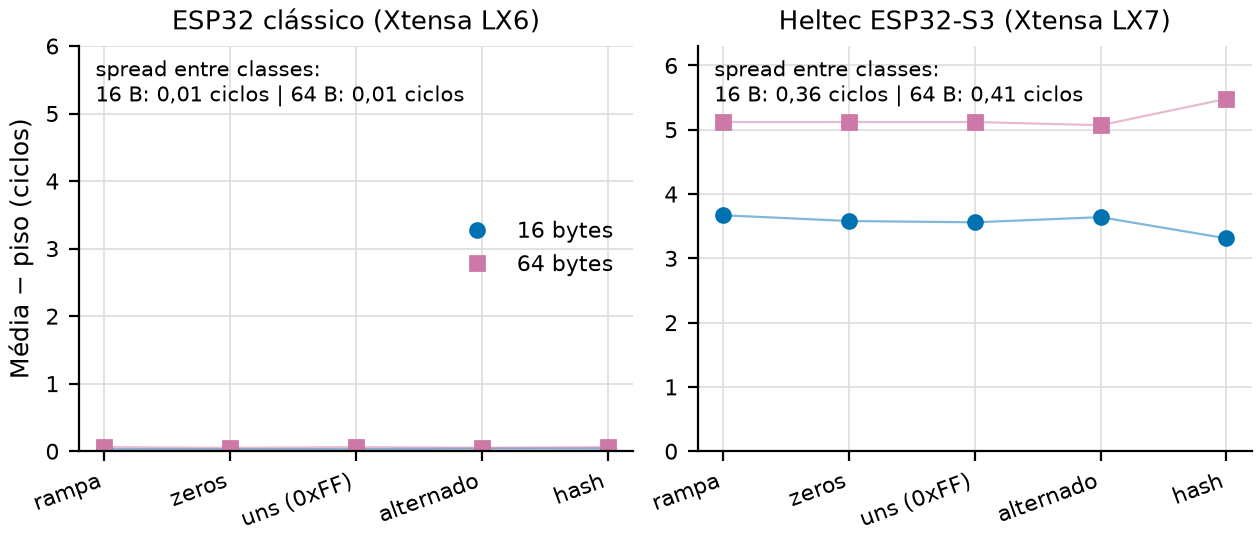
\includegraphics[width=\textwidth]{figuras/bench_tempo_constante.png}
  \end{center}
  \legend{Fonte: elaborado pelos autores.}
\end{figure}

%%%%%%%%%%%%%%%%%%%%%%%%%%%%%%%%%%%%%%%%%%%%%%%%%%%%%%

\subsection{Comparativo com AES-128-GCM}

Para responder à questão central levantada na Seção 2.2.2, se a migração para criptografia leve em software traz vantagem real frente ao acelerador de \textit{hardware} já presente nas placas comerciais, comparou-se o Ascon-128a (software) com o AES-128-GCM (\textit{Galois/Counter Mode}) na mesma execução e sob as mesmas condições, nas duas placas. O AES-GCM foi avaliado por meio da biblioteca \textit{mbedTLS} do próprio \textit{core} do ESP32, com a chave fixada uma vez por execução, como num nó que possui uma única chave. Nos dois chips, apenas o bloco AES é executado no acelerador de \textit{hardware}. A autenticação (GHASH) permanece em \textit{software}, e nenhum dos dois declara suporte a GCM no acelerador \cite{espressif2026idf}. As placas diferem no caminho pelo qual o driver alimenta o acelerador. No ESP32 clássico a CPU escreve e lê um bloco de 16 bytes por vez, e no ESP32-S3 o driver usa DMA \cite{espressif2026idf}.

Cada algoritmo foi medido pelo piso de 2.000 medidas, alternando-se os dois na mesma execução, em 100 execuções por tamanho, para cifragem e decifragem. A Tabela~\ref{tab:comparativo_aes} apresenta os pisos da cifragem e a razão entre eles, e a Tabela~\ref{tab:comparativo_aes_dec} faz o mesmo para a decifragem. A decifragem interessa por conta própria, pois é a operação que o receptor executa para cada pacote de cada nó. A Figura~\ref{fig:bench_ciclos_tamanho} mostra as mesmas curvas, com a cifragem acima e a decifragem abaixo.

\begin{table}[htb]
\centering
\caption{Piso de ciclos da cifragem do Ascon-128a (software) e do AES-128-GCM (\textit{mbedTLS}), nas duas placas, e razão AES/Ascon}
\label{tab:comparativo_aes}
\begin{tabular}{rrrrrrr}
\hline
\textbf{Payload} & \multicolumn{3}{c}{\textbf{ESP32 clássico}} & \multicolumn{3}{c}{\textbf{ESP32-S3}} \\
 & \textbf{Ascon} & \textbf{AES-GCM} & \textbf{razão} & \textbf{Ascon} & \textbf{AES-GCM} & \textbf{razão} \\
\hline
0 bytes  & 5.037 & 6.497  & 1,29 & 4.603 & 10.465 & 2,27 \\
2 bytes  & 5.181 & 8.174  & 1,58 & 4.722 & 16.556 & 3,51 \\
16 bytes & 6.134 & 8.603  & 1,40 & 5.639 & 19.473 & 3,45 \\
23 bytes & 6.521 & 10.454 & 1,60 & 5.960 & 20.920 & 3,51 \\
32 bytes & 7.231 & 10.712 & 1,48 & 6.675 & 20.398 & 3,06 \\
64 bytes & 9.425 & 14.930 & 1,58 & 8.747 & 22.267 & 2,55 \\
\hline
\end{tabular}
\legend{Fonte: elaborado pelos autores.}
\end{table}

\begin{table}[htb]
\centering
\caption{Piso de ciclos da decifragem do Ascon-128a (software) e do AES-128-GCM (\textit{mbedTLS}), nas duas placas, e razão AES/Ascon}
\label{tab:comparativo_aes_dec}
\begin{tabular}{rrrrrrr}
\hline
\textbf{Payload} & \multicolumn{3}{c}{\textbf{ESP32 clássico}} & \multicolumn{3}{c}{\textbf{ESP32-S3}} \\
 & \textbf{Ascon} & \textbf{AES-GCM} & \textbf{razão} & \textbf{Ascon} & \textbf{AES-GCM} & \textbf{razão} \\
\hline
0 bytes  & 5.256  & 6.908  & 1,31 & 4.755 & 10.814 & 2,27 \\
2 bytes  & 5.366  & 8.585  & 1,60 & 4.841 & 16.903 & 3,49 \\
16 bytes & 6.646  & 9.014  & 1,36 & 5.959 & 19.820 & 3,33 \\
23 bytes & 6.989  & 10.867 & 1,55 & 6.212 & 21.269 & 3,42 \\
32 bytes & 8.036  & 11.123 & 1,38 & 7.163 & 20.745 & 2,90 \\
64 bytes & 10.816 & 15.341 & 1,42 & 9.571 & 22.616 & 2,36 \\
\hline
\end{tabular}
\legend{Fonte: elaborado pelos autores.}
\end{table}

\begin{figure}[htb]
  \caption{\label{fig:bench_ciclos_tamanho}Piso de ciclos da cifragem (acima) e da decifragem (abaixo) por tamanho de \textit{payload}, Ascon-128a e AES-128-GCM, nas duas placas}
  \begin{center}
      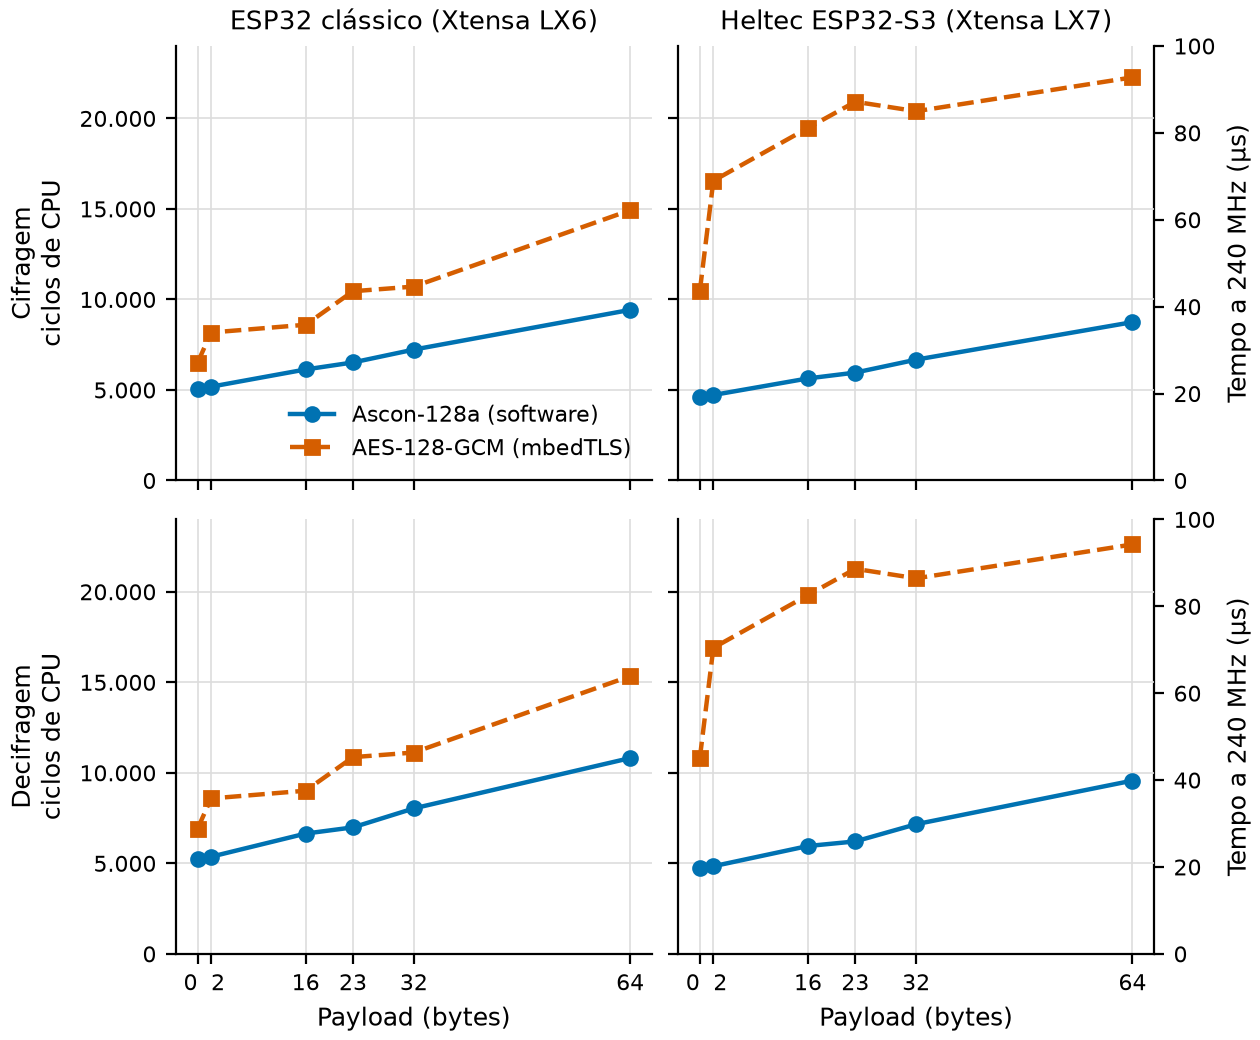
\includegraphics[width=\textwidth]{figuras/bench_ciclos_tamanho.png}
  \end{center}
  \legend{Fonte: elaborado pelos autores.}
\end{figure}

O Ascon-128a foi mais rápido que o AES-128-GCM em todas as 1.200 execuções de cada placa (seis tamanhos, cifragem e decifragem, 100 execuções). No ESP32 clássico a vantagem vai de 1,29 vez, com o \textit{payload} vazio, a 1,60 vez, em 23 bytes, e tende a crescer com o número de blocos. Na decifragem, vai de 1,31 a 1,60. No ESP32-S3 ela vai de 2,27 a 3,51 vezes na cifragem e de 2,27 a 3,49 na decifragem, e diminui com o tamanho (Figura~\ref{fig:bench_razao_tamanho}). As duas tendências têm a mesma origem, o custo por bloco e a parcela fixa de cada caminho do AES, examinados a seguir.

\begin{figure}[htb]
  \caption{\label{fig:bench_razao_tamanho}Razão entre os pisos de ciclos do AES-128-GCM e do Ascon-128a, na cifragem e na decifragem, por tamanho de \textit{payload}}
  \begin{center}
      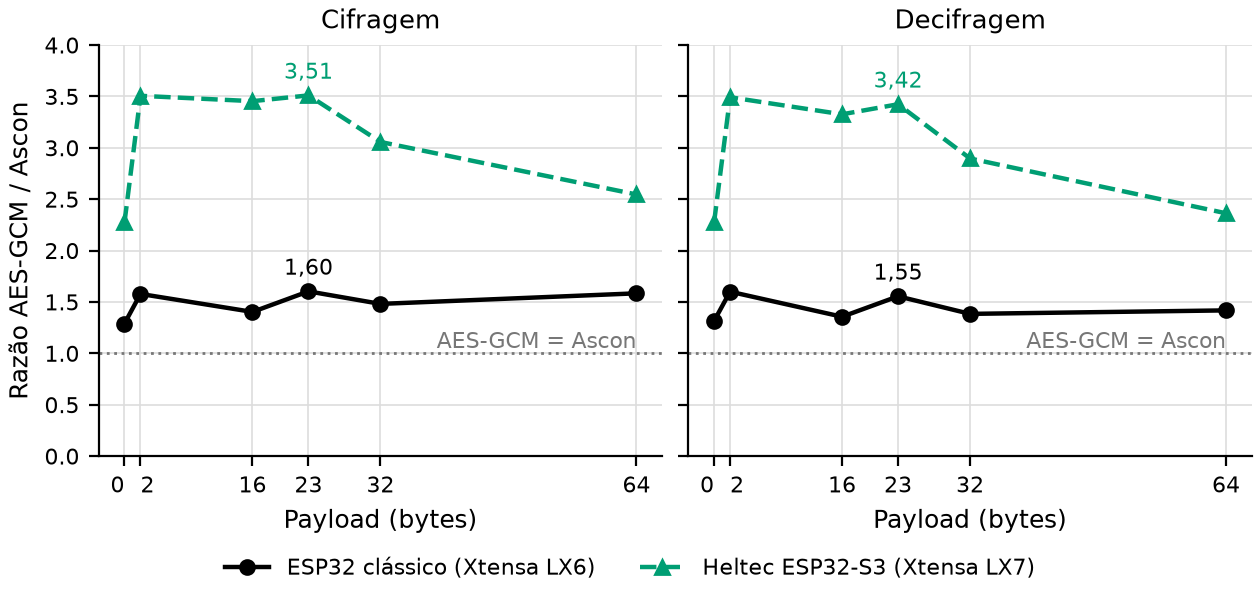
\includegraphics[width=\textwidth]{figuras/bench_razao_tamanho.png}
  \end{center}
  \legend{Fonte: elaborado pelos autores.}
\end{figure}

O AES-GCM é a cifragem em modo contador (CTR) mais o cálculo da \textit{tag} pelo GHASH \cite{dworkin2007gcm}, e no ESP-IDF a rotina de GCM reutiliza a de CTR \cite{espressif2026idf}. Assim, a diferença entre os custos por bloco dos dois modos é o GHASH, e por isso mediu-se também o AES-128-CTR. Ele entra aqui só como instrumento de medição, pois sem autenticação não atenderia ao requisito desta camada. A Figura~\ref{fig:bench_decomposicao_bloco} resume a decomposição. No ESP32 clássico, cada bloco adicional de 16 bytes custa 825 ciclos no AES-CTR e 2.109 no AES-GCM, logo 1.284 ciclos no GHASH. No ESP32-S3, são 49 ciclos no CTR, 931 no GCM e 882 no GHASH. Em ambos, o GHASH sozinho custa mais do que o Ascon-128a gasta para cifrar e autenticar um bloco inteiro (1.097 e 1.036 ciclos). Mesmo os 825 ciclos por bloco do CTR no ESP32 clássico estão longe do núcleo do acelerador, ao qual o manual do fabricante atribui 11 a 15 ciclos de \textit{clock} por bloco \cite{espressif2026trm}. O restante é gasto pelo \textit{software} do driver e pela transferência dos dados entre a CPU e o periférico.

\begin{figure}[htb]
  \caption{\label{fig:bench_decomposicao_bloco}Custo marginal por bloco de 16 bytes: Ascon-128a completo e AES-128-GCM decomposto em cifra AES (CTR) e GHASH, nas duas placas}
  \begin{center}
      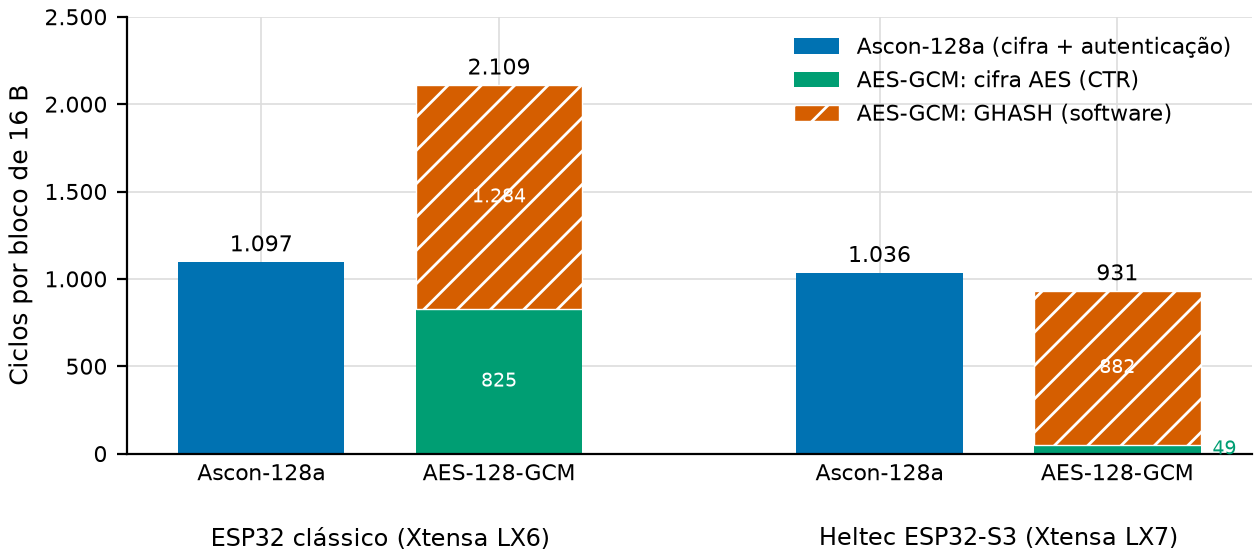
\includegraphics[width=\textwidth]{figuras/bench_decomposicao_bloco.png}
  \end{center}
  \legend{Fonte: elaborado pelos autores.}
\end{figure}

No ESP32-S3, o caminho por DMA reduz o custo por bloco a 49 ciclos, mas cobra caro por chamada. Cada transferência exige preparar e depois liberar o canal de DMA \cite{espressif2026idf}, e o AES-CTR de 16 bytes custou 8.218 ciclos, contra 2.316 no ESP32 clássico. Como o GCM faz duas transferências por mensagem, uma para os dados e outra para a \textit{tag}, sua parcela fixa chega a cerca de 18.500 ciclos, e é isso que torna o AES-GCM 3,5 vezes mais lento que o Ascon na mensagem de 23 bytes. O bloco parcial recebe tratamento à parte no driver, o que ajuda a explicar 23 bytes terem custado mais que 32 (20.920 contra 20.398 ciclos). Os pisos do AES-GCM no ESP32-S3 variaram até 8 ciclos entre as 100 execuções, cerca de 0,04\%, e no ESP32 clássico no máximo 2. Os do Ascon não variaram em nenhum caso.

Para os pacotes pequenos típicos de redes LoRaWAN, portanto, a criptografia leve em software não apenas dispensa o acelerador de \textit{hardware} como o supera em latência nos dois chips, e por margem maior justamente na placa de implantação, mantendo ainda a ausência de alocação dinâmica, que o AES não mantém no ESP32-S3. Ressalva-se que o resultado se refere ao AES-GCM do \textit{mbedTLS} pelo \textit{port} da Espressif, nas versões indicadas. Entre os alvos do ESP-IDF, apenas o ESP32-S2 declara aceleração de GCM, e ainda assim parcial, pois o GHASH permanece em \textit{software}, de modo que não se espera que a comparação se inverta nas demais variantes \cite{espressif2026idf}. A avaliação de consumo energético dessa mesma comparação, descrita na Seção 3.4.4, complementará esta análise.

%%%%%%%%%%%%%%%%%%%%%%%%%%%%%%%%%%%%%%%%%%%%%%%%%%%%%%

\subsection{Integração no enlace LoRa: biblioteca \textit{AsconSecure}}
\label{subsec:asconsecure}

As seções anteriores validam o algoritmo. Para que a frente de comunicação o utilize sem lidar com chave, \textit{nonce} ou contador, a camada de segurança foi empacotada como uma biblioteca Arduino, a \textit{AsconSecure}, na pasta \texttt{ascon-lora} do repositório. Ela reúne três papéis. O provisionamento do nó é feito uma vez na bancada, o emissor cifra no nó sensor, e o receptor decifra no \textit{gateway}. Para a aplicação, o uso se resume a uma chamada para cifrar e uma para decifrar. Quando a operação falha, o resultado não contém bytes, e não há o que transmitir ou consumir.

Cada mensagem no ar é formada por um contador de 4 bytes, pelo texto cifrado e pela \textit{tag} de 16 bytes, o que acrescenta 20 bytes fixos ao \textit{payload}. O \textit{nonce} de 128 bits é composto por um prefixo de 12 bytes, gerado no provisionamento e conhecido pelo receptor, seguido do contador, e só o contador viaja. Ele não precisa de proteção à parte, pois alterá-lo em trânsito altera o \textit{nonce} e invalida a \textit{tag}, como mostrou a Seção~\ref{subsec:aead_resultados}.

A chave de 128 bits e o prefixo são gerados no próprio nó, pelo CTR\_DRBG da \textit{mbedTLS} alimentado pelo gerador de \textit{hardware} do ESP32 (RF3 e RF4), e gravados na memória não volátil (NVS). A saída do gerador é usada diretamente como chave, o caso $V$ nulo da operação $K = U \oplus V$ do SP 800-133r2 \cite{barker2020nist133}. Um cuidado vem da documentação do ESP-IDF. O gerador de \textit{hardware} só produz números verdadeiramente aleatórios com o Wi-Fi ou o Bluetooth ligados, ou com uma fonte interna de entropia habilitada por \texttt{bootloader\_random\_enable()}, e fora dessas condições sua saída deve ser considerada apenas pseudoaleatória \cite{espressif2026random}. Como o nó não usa Wi-Fi nem Bluetooth, a biblioteca habilita essa fonte durante a geração da chave e a desabilita em seguida. A mesma documentação exige que isso ocorra antes de o conversor analógico-digital ou o rádio serem iniciados, e por isso a geração da chave é uma etapa própria, o provisionamento, separada da inicialização do emissor. Como cada nó gera a própria chave, nenhuma é compartilhada (RF6), e o \textit{gateway} não tem chave própria, apenas guarda a de cada nó que escuta.

A unicidade do \textit{nonce} (RNF2 e RF7) vem de um contador de 32 bits persistido na NVS. Para não gravar a \textit{flash} a cada mensagem, o emissor reserva 32 valores por vez, gravando o valor 32 posições à frente antes de usar a faixa, e só volta a gravar quando ela se esgota. Após uma reinicialização, o contador recomeça do valor reservado, pois tudo abaixo dele pode ter ido ao ar. Uma queda de energia descarta até 32 valores, mas nunca repete um, e diante de $2^{32}$ valores o descarte é irrelevante. O contador pertence a esta camada e independe do contador de quadros do LoRaWAN, como exige o RF7. Perto do fim, a cifragem é recusada antes que o valor dê a volta, e a saída é reprovisionar o nó.

No \textit{gateway}, o receptor guarda na NVS, para cada nó, o maior contador já aceito. A decifragem verifica primeiro a \textit{tag} e depois o contador. Um pacote com \textit{tag} inválida é descartado antes de qualquer consulta ao estado, para que um pacote forjado com contador alto não bloqueie o nó legítimo, e um pacote autêntico com contador igual ou menor que o último aceito é descartado como repetição (RF9). O novo contador é gravado antes de a mensagem ser entregue. Se a gravação falhar, a mensagem é descartada, pois entregar sem gravar permitiria, após um reinício, aceitar de novo tudo o que chegou no intervalo. O texto claro fica num \textit{buffer} interno e só é copiado à aplicação depois das duas verificações, o que estende ao código de integração a garantia do RF8. O registro é indexado por uma impressão da chave, os 8 primeiros bytes do \textit{hash} Ascon de chave e prefixo, e não pelo número do nó, para que um erro de configuração, como registrar o mesmo nó sob dois números, não reabra o histórico à repetição.

A renovação da chave (RF5) é feita por novo provisionamento, em que se apaga o estado do nó, gera-se nele uma chave nova e substitui-se o registro no receptor. Nenhuma chave trafega pelo ar.

Os \textit{buffers} da biblioteca têm tamanho fixo e a cifragem não aloca memória dinâmica, como medido na Seção~\ref{subsec:memoria_tempo}. O acesso à NVS, feito pelo ESP-IDF, cria e libera um objeto em memória dinâmica a cada gravação \cite{espressif2026idf}, isso ocorre fora da cifragem, uma vez a cada 32 mensagens no emissor e a cada mensagem aceita no receptor. A Tabela~\ref{tab:asconsecure_requisitos} resume o atendimento aos requisitos da Seção~\ref{sec:requisitos_seguranca}.

\begin{table}[htb]
\centering
\caption{Requisitos da Seção~\ref{sec:requisitos_seguranca} atendidos pela biblioteca \textit{AsconSecure}}
\label{tab:asconsecure_requisitos}
\begin{tabular}{lp{10cm}}
\hline
\textbf{Requisito} & \textbf{Como é atendido} \\
\hline
RF2, RF3, RF4 & Chave gerada no nó pelo CTR\_DRBG da \textit{mbedTLS}, semeado pelo gerador de \textit{hardware} com a fonte interna de entropia habilitada, com $V$ nulo. \\
RF5           & Renovação por novo provisionamento, nenhuma chave trafega pelo ar. \\
RF6           & Cada nó gera a própria chave e o \textit{gateway} guarda uma por nó. \\
RF7           & Contador de 32 bits na NVS, reservado em blocos de 32 antes do uso, independente do contador de quadros do LoRaWAN. \\
RF8           & Texto claro só é copiado à aplicação após \textit{tag} e contador aprovados. \\
RF9           & Receptor descarta contador igual ou menor que o último aceito, gravado antes da entrega. \\
RNF1          & Entropia bruta condicionada pelo CTR\_DRBG. \\
RNF2          & Chave guardada na NVS do nó e apagada da RAM ao ser descartada, e \textit{nonce} único pelo contador. \\
RNF5          & \textit{Tag} de 16 bytes, sem truncamento. \\
RNF6, RNF7    & \textit{Buffers} de tamanho fixo e cifragem sem alocação dinâmica. \\
\hline
\end{tabular}
\legend{Fonte: elaborado pelos autores.}
\end{table}

Dois limites ficam registrados. O provisionamento imprime a chave na porta serial para ser copiada ao receptor, o que só é aceitável na bancada, com o nó sob controle físico. E o registro anti-repetição vive na NVS do \textit{gateway}. Se ela for apagada, mensagens antigas voltam a ser aceitas, cada uma no máximo uma vez, até que o contador do nó legítimo as ultrapasse. A execução da biblioteca nas placas ainda não foi realizada e será incorporada quando concluída.

%%%%%%%%%%%%%%%%%%%%%%%%%%%%%%%%%%%%%%%%%%%%%%%%%%%%%%

\subsection{Limitações das Medições}
\label{subsec:limitacoes_ascon}

Os resultados desta seção valem para as condições em que foram obtidos. As placas foram o ESP32 clássico e o ESP32-S3 da Heltec, a 240~MHz, com o \textit{core} arduino-esp32 3.3.11 sobre o ESP-IDF 5.5.5 e a biblioteca \textit{ascon-suite} na versão indicada na Seção~\ref{subsec:biblioteca-ascon}. Nada aqui se generaliza para outras famílias de microcontroladores, e o próprio fabricante observa que a 240~MHz o acelerador de AES não oferece ganho sobre o AES em \textit{software} \cite{espressif2026idf}, o que faz parte do contexto da comparação. A variante medida é o Ascon-128a versão 1.2, e não o Ascon-AEAD128 do SP 800-232, cujas diferenças se limitam a constantes, como mostra a Tabela~\ref{tab:parametros_ascon}. Os \textit{payloads} foram de 0 a 64 bytes, o modelo linear de custo foi validado nessa faixa e não foi verificado para mensagens maiores. A resistência a canais laterais foi avaliada apenas quanto ao tempo de execução, consumo de potência e emissão eletromagnética ficam como trabalho futuro. O tempo no ar é calculado pela fórmula do fabricante do rádio, não medido. Por fim, a montagem do laboratório usa LoRa ponto a ponto, sem a pilha LoRaWAN, e toma do protocolo apenas os limites de \textit{payload} e a configuração do rádio, de modo que a proteção da camada MAC do LoRaWAN não faz parte do que foi medido.
